This work explores the prospects of deep recurrent end-to-end architectures applied to speech recognition. Complementary aspects of developing speech recognition systems are eliminated by focusing on end-to-end speech units as a two-step process requiring a Connectionist Temporal Character Classification (CTCC)\cite{graves2006connectionist} model and Language Model (LM) rather than a three-step process requiring an Acoustic model(AM), LM and phonetic dictionary. A two-step process rather than a three-step process is particularly desirable for low resource languages as less effort is required developing fewer simplified models.

Earlier in chapter one, deep learning was defined as a type of representational learning whereby different levels of complexity are captured in internal layer-wise encapsulations. It has also been noted that layer-wise stacking of neural and neural network type architectures such as the Restricted Boltzmann Machine (RBM) deep belief networks (DBMs) are used to implement such representations. In this chapter, the end-to-end Bi-directional Recurrent Neural Network model is described. Here, the development of the features using the deep scattering convolution network is first elaborated on. The model parameters and architecture is described and the decoding algorithm is detailed.

\section{Deep Scattering Features}
The fast wavelet transformed is derived in Chapter 4 from a low pass filter and a high pass filter.  The speech features used in this research using a deep scattering network 2 layers deep was created using the wavelet modulus operator comprising a low pass filter and a band pass filter.   Hyper parameters of the system included the window period for each sampled sub section, T;  The Q-band value for the band pass filter and the number of wavelets $J$ at each scattering layer for the total number of layers, $M=2$.

The matlab scatnet toolbox \citep{anden2014scatnet}, used to determine the scatter coefficient features for this research, provides optimal values for hyper parameters for audio signal processing into scatter features.  In this regime the value for the hyper parameter $T$, the number of samples per window, = $512$ samples per window. This approximates a window of $50 milliseconds$ for the audio signals sampled at $8000 Hz$.  For the first scattering layer the parameter, $Q=8$ and for the second scattering layer, the $Q=1$.  Finally $J$ is pre-calculated based on the value of $T$.  These after scatnet processing, eventually produce a feature-vector $165$ coefficients long.  These feature vectors in turn are used as inputs to the bi-direction neural network model whose architecture is explained in the succeeding sections.

\section{CTCC-BiRNN Architecture}
The core of the system is a bidirectional recurrent neural network (BiRNN) trained to ingest scatter coefficients described in the previous section, in order to generate English text transcriptions.  An end-to-end system therefore specifies that utterances $x$ and the corresponding label $y$ be sampled from a training set such that the sample $S = {(x^{(1)}, y^{(1)}), (x^{(2)}, y^{(2)}), . . .}$.   In our end-to-end model, each utterance, $x^{(i)}$ is a time-window consisting of $T^{(i)}$ samples.  Each window passes through a scattering transform to yield an input of vector of p features; so   $x^{(i)}_{t,p}$ denotes the $p$-th feature in a scatter transform at time .  

GPU training of the speech model architecture developed above was done using Mozilla deepspeech \cite{mozilla/deepspeech_2019} CTC bi-directional RNN implementation along with the accompanying Mozilla Common voice dataset  \cite{common voice by mozilla_2019}.  The Common Voice Dataset project consists of voice samples in short recordings approximately $4$ seconds each.  The complete dataset is about $250$ hours of recording divided into training, test and development subsets.  The BiRNN, given the input sequence, $x$, outputs a sequence of probabilities $y_t=\mathbb{P}(c_t|x)$,  where $c_t \in a,b,c,\dots,z,space,apostrophe,blank$. 

The actual architecture of our core Bi-RNN is similar to the deepspeech system described in \cite{hannun2014deep}. This structure consists of a 5 hidden layers and one output layer.  The first three layers are regular DNNs followed by a bi-directional recurrent layer. As such, the output of the first three layers are computed by:
\begin{equation}
    h^{(l)}_t = g(W^{(l)} h^{(l−1)}_t + b^{(l)})\label{ch06_01_l1-3}
\end{equation}

$g(\cdot) = min\{max\{0,z\},20\}$  is the clipped rectified linear unit and $W^{(l)},b^{(l)}$ are weight matrix and bias parameters for layer  as described in sections \ref{dnn} and \ref{deepspeech} respectively.

It was shown in chapter \ref{ch3RNN} the recurrent layer comprise a forward and backward RNNs whose equations are repeated here for reference
\begin{equation}
    h^{(f)}_t = g(W^{(4)} h^{(3)}_t + W^{(f)}_r h^{(f)}_{t−1} + b^{(4)})
    \label{ch06_02_fwd}
\end{equation}
\begin{equation}
h^{(b)}_t = g(W^{(4)} h^{(3)}_t + W^{(b)}_r h^{(b)}_{t+1} + b^{(4)})    \label{ch06_03_bwd}
\end{equation}

Consequently, $h^{(f)}$ is the sequential computation from $t=1$ to $t=T^{(i)}$ for the $i$-th utterance and $h^{(b)}$ is the reverse computation from $t=T^{(i)}$ to $t=1$.  In addition the output from layer five is summarily given as the combined outputs from the recurrent layer:
\begin{equation}
h^{(5)} = g(W^{(5)} h^{(4)} + b^{(5)})    \label{ch06_04_l5}
\end{equation}
where $h^{(4)} = h^{(f)} + h^{(b)}$. The output of the Bi-RNN on layer 6 is a standard soft-max layer that outputs a predicted character over probabilities for each time slice $t$ and character $k$ in the alphabet:
\begin{equation}
h^{(6)}_{t,k} = \hat{y}_{t,k} \equiv \mathbb{P}(c_t = k \mid x) = \frac{\exp{ \left( (W^{(6)} h^{(5)}_t)_k + b^{(6)}_k \right)}}{\sum_j \exp{\left( (W^{(6)} h^{(5)}_t)_j + b^{(6)}_j \right)}})    \label{ch06_05_l6}
\end{equation}

$b^{(6)}_k$ takes on the -th bias and $(W^{(6)} h^{(5)}_t)_k$ is the matrix product of the $k$-th element.  The error of the outputs are then computed using the CTC loss function \cite{graves_2014} described in chapter \ref{ch3DNN}.  A summary of our model is illustrated in figure \ref{fig_6_1_ctc_scatter}.
\begin{figure}
\centering
  % Requires \usepackage{graphicx}
  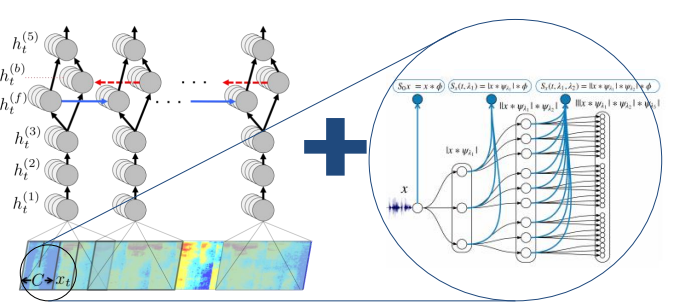
\includegraphics[width=14cm]{thesis/images/ctc_scatter.png}\\
  \caption{Deep scattering Bi-RNN Model} \label{fig_6_1_ctc_scatter}
\end{figure}

\section{Model Hyper parameters}
The hidden layer matrix for each layer comprised 1024 hidden units (6.6M free parameters).  The weights are initialised from a uniform random distribution having a standard deviation of 0.046875.  Adam optimisation algorithm \citep{kingma2014adam} was used with initial learning rate of , and a momentum of 0.95 was deployed to optimise the learning rate.

The network for network was trained for a total of five to fifty epochs over the training set for experiments conducted. The training time for Python GPU implementation is shown in Table \ref{ch06_tab_01}.  For decoding with prefix search we use a beam size of 200 and cross-validated with a held-out set to find a good setting of the parameters α and β. Table 1 shows word error rates for various GPU configurations and audio dataset sizes


\begin{table}
  \caption{GPU Experiments}
  \label{tab_c6_01_training}
\begin{tabular}{lccc}
\toprule
Experiment & Hours of speech & Total training time & Estimated training\\
\midrule
1. 2xGPU 10GB RAM & 1 & 7 days & Completed\\
2. 2xGPU 10GB RAM & 10 & 150+ days & 300 days\\
3. 5xGPU 15GB RAM & 10 & 17 hours & Completed\\
4. 5xGPU 15GB RAM & 40 & 5+ days & 10 days\\
\bottomrule
\end{tabular}
\end{table}
\section{CTC Decoding}

Assuming an input of length $T$, the output of the neural network will be $p(c|c_t)$ for $t=1,\dots,T$. Again $p(c|c_t)$ is a distribution over possible characters in alphabet $\Sigma$, which includes the blank symbol, given audio input $x_t$. In order to recover a character string from the output of the neural network, as a first approximation, we take the $arg\max$ at each time step. Let $S=(s_1,\dots,s_T)$ be the character sequence where $s_t=arg\max_{c\in\Sigma}p(c|x_t)$. The sequence $S$ is mapped to a transcription by collapsing repeat characters and removing blanks. This gives a sequence which can be scored against reference transcription using both CER and WER.

The first approximation lacks the ability to include the constraint of either a lexicon or language model. We propose a generic algorithm which is capable of incorporating such constraints. Taking X to be acoustic input of time T, we seek a transcription W which maximises the probability.
The first approximation lacks the ability to include the constraint of either a lexicon or language model. We propose a generic algorithm which is capable of incorporating such constraints. Taking X to be acoustic input of time T, we seek a transcription W which maximises the probability.
\begin{equation}
$$p_{net}(W;X)p_{lm}(W)$$
\label{eqn_c6_brnn06}
\end{equation}

Here the overall probability of the transcription is modeled as the product of two factors: pnet given by the network and plm given by the language model prior. In practice the prior plm(W), when given by an n-gram language model, is too constraining and thus we down-weight it and include a word insertion penalty or bonus as
\begin{equation}
p_{net}(W;X)p_{lm}(W)^\alpha|W|^\beta
\label{eqn_c6_brnn07}
\end{equation}

Algorithm 1 attempts to find a word string W which maximizes equation 8. The algorithm maintains two separate probabilities for each prefix,  and . Respectively, these are the probability of the prefix ending in blank or not ending in blank given the first  time steps of the audio input .

Algorithm 1 Prefix Beam Search: The algorithm initializes the previous set of prefixes  to the empty string. For each time step and every prefix  currently in , we propose adding a character from the alphabet  to the prefix. If the character is a blank, we do not extend the prefix. If the character is a space, we incorporate the language model constraint. Otherwise we extend the prefix and incorporate the output of the network. All new active prefixes are added to . We then set  to include only the  most probable prefixes of . The output is the 1 most probable transcript, although the this can easily be extended to return an n-best list.

The sets  and  maintain a list of active prefixes at the previous time step and a proposed prefixes at the next time step respectively. Note that the size of  is never larger than the beam width . The overall probability of a prefix is the product of a word insertion term and the sum of the blank and non-black ending probabilities.
\begin{equation}
p(\ell;x_{1:t})=(p_b(\ell;x_{1:6})+p_{nb}(\ell;x_{1:t}))|W(\ell)|^\beta
\label{eqn_c6_brnn08}
\end{equation}

Where  is a set of words in the sequence . When taking the  most probable prefixes of , we sort each prefix using the probability given in equation (\ref{eqn_c6_brnn08}).
The variable  is the last character in the label sequence . The function , which converts  into a string of words, segments the sequence  at each space character and truncates any characters trailing the last space.

We incorporate a lexicon or language model constraint by including the probability  whenever the algorithm proposes appending a space character to . By setting  to 1 if the last word of  is in the lexicon and 0 otherwise, the probability acts a a constraint forcing all character strings to consists of words only in the lexicon.  Furthermore,  can represent an n-gram language model by considering only the last n-1 words in .

\section{Results}
A total of four experiments were carried out on two different GPU configurations. A set of experiments was performed a GPU configuration consisting of 2 GPUs having a total of 10 gigabytes of memory. The second set of experiments was carried out on a GPU configuration comprising 5 GPUs having a total of 15 gigabytes of memory.  For each configuration two experiments were carried out on a small subset of the dataset then on a larger subset of the common voice dataset being used.   The various GPU configurations along with the training times is shown in Table 1.

The output of the training produced mostly gibberish when trained in both configurations using only just one hour of training data.  Training loss reduced significantly once the data was increased to ten hours of training.  However word error rates (WER) only showed improvement on the 40 hours dataset.

The results showed that the training of the model was heading towards a very slow convergence as indicated by the slow decrements in training loss.  However, we perceive that given the complete dataset to train the model will not only converge but show improvements in word error rates.

